\documentclass[a4paper]{jsarticle}

%======================================================================
%		論文のタイトル,著者,日付
%======================================================================

\title{\Huge マルチメディア信号処理\\\huge 第1回レポート\vspace{120mm}}
\author{\Large 濱崎 直紀 \and \Large 永井 智之 \and \Large 中尾 文亮\vspace{30mm}}
\date{令和元年6月5日}

%======================================================================
%		マクロの読み込みとコマンドの定義
%======================================================================

\usepackage{graphicx}       % eps file を張り付けるのに必要
%\usepackage[dvipdfmx]{graphicx}     % png等の画像を貼りつけるのに必要
\usepackage{bm}     % 太字を書くのに必要
\usepackage{here}       % その場所に画像を入れるのに必要
\usepackage{comment}        % コメントを挟むのに必要
\usepackage{listings}      % ソースコードを表示するのに必要
\usepackage{jlisting}       % ソースコード内に日本語のコメントアウトがある場合必要(TEX Live の場合,別途ダウンロードが必要)

%======================================================================
%		本文
%======================================================================

\begin{document}

\begin{titlepage}
\maketitle
\thispagestyle{empty}
\end{titlepage}

\section{問題}
一部重なりのある2枚の画像を,大きさ・位置・角度を正しく合わせてつなげるプログラムの作成.

\subsection{課題内容}
与えられた一部重なりのある2枚の画像をimage1,image2とした場合に,image1を基準に,2枚の画像が重なるようにimage2の水平・垂直方向の移動量,回転角および拡大率を算出するプログラムを作成する.
ただし,以下の条件があるものとする.
\begin{itemize}
    \item 画像の大きさは幅640以下,高さ480以下
    \item 水平・垂直方向の移動量は画像の幅,高さを超えない
    \item 回転角は時計回り,反時計回りともに15度未満
    \item 拡大倍率は0.5以上2.0以下
\end{itemize}

\subsection{補足}
実際のプログラムに関しては,レポート末尾に付録として記載.

\section{アルゴリズム(FAST)の概要}
私たちの班は,問題解決のアルゴリズムとしてFASTを用いた.
FASTの概要を以下に示す.

\subsection{原理}
FASTによる特徴量抽出の仕組みは以下のようなものである。
\begin{enumerate}
    \item あるピクセルにおける輝度値を$I_p$とする.
    \item 適当な閾値$t$を選ぶ.
    \item 周囲の16ピクセルに置いて,その輝度値が$I_p-t$より小さいか,$I_p+t$より大きいか,そのどちらでもないかを判定する.
    輝度値が$I_p-t$より小さいピクセルか,$I_p+t$より大きいピクセルがある数$n$以上の場合,その点を特徴点(corner)として抽出する.
\end{enumerate}
\begin{figure}[H]
    \begin{center}
        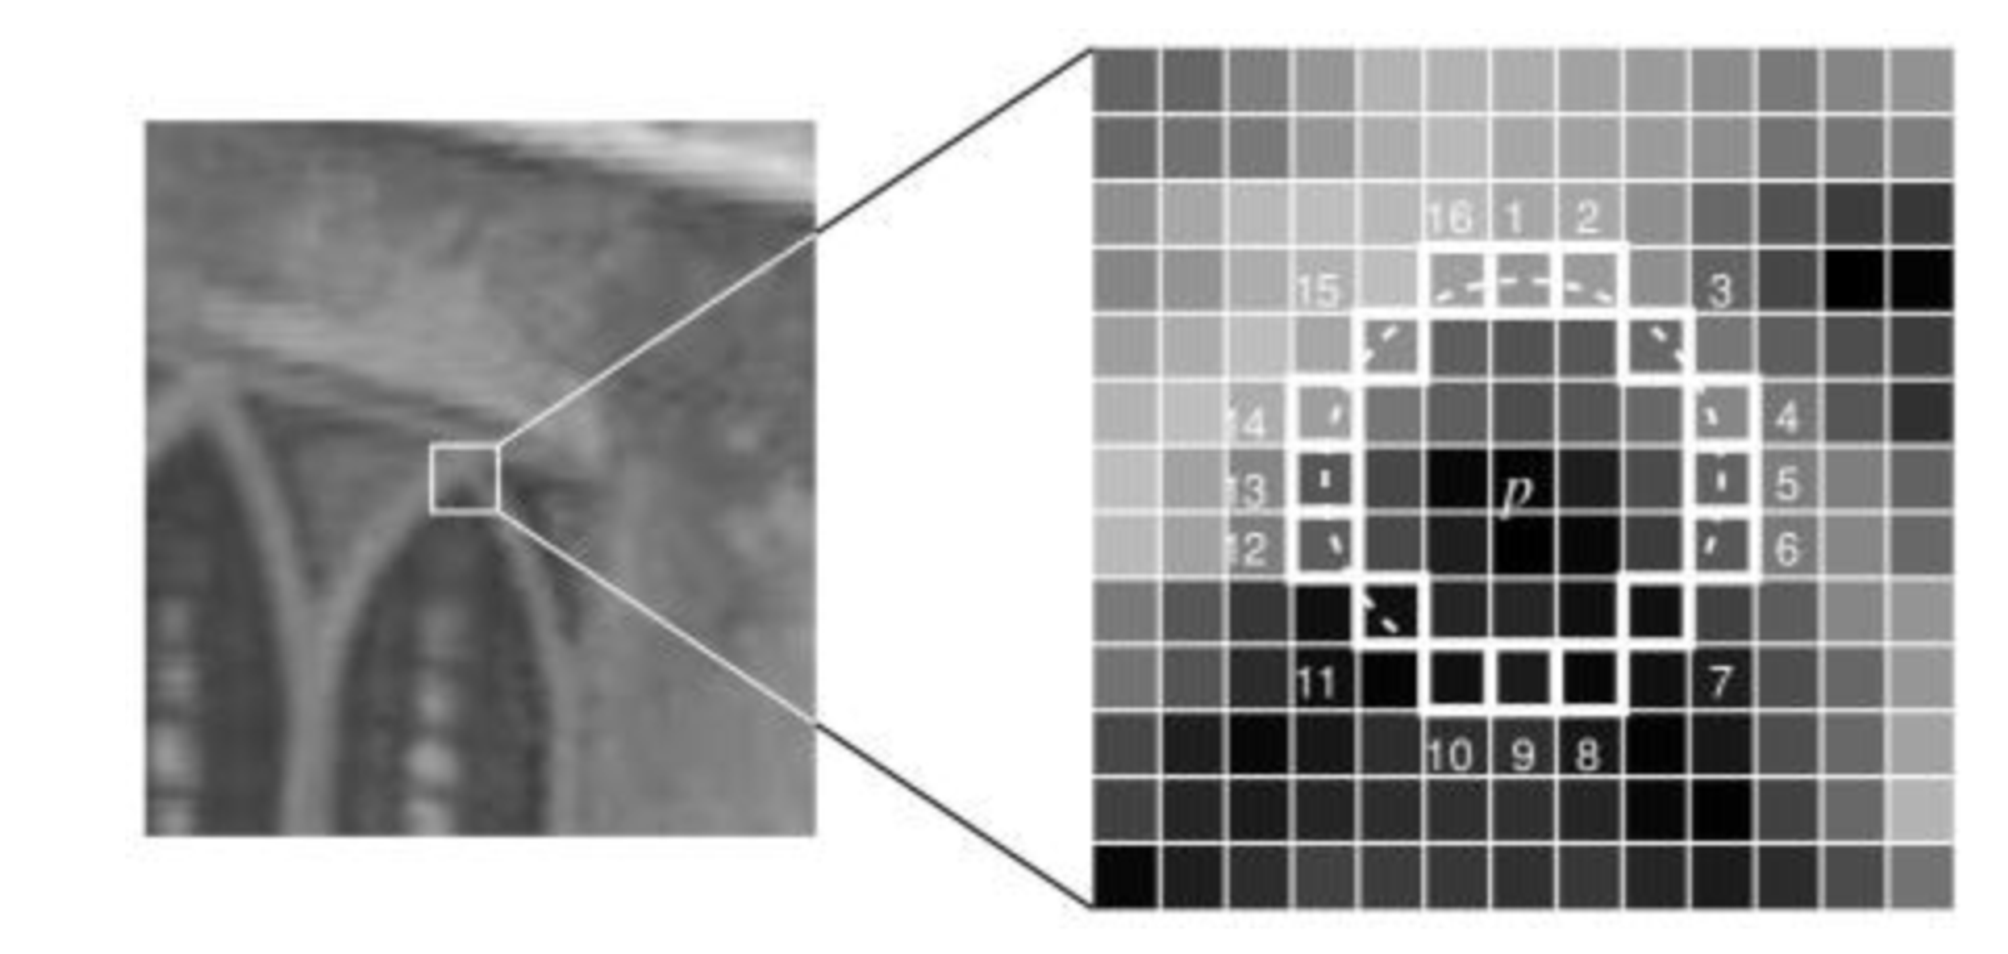
\includegraphics[width=120mm]{./figures/overview/fig1.eps}
    \end{center}
\end{figure}

\subsection{実装}
\begin{itemize}
    \setlength{\itemsep}{5mm}
    \item FASTの実装\par
    \vspace{1mm}
    \quad
    前節で述べたFASTの仕組みを以下のように実装した.
    なお,$t=50$,$n=12$とした.
    $n$の値は,FASTにおける高速化プログラムを意識した設定であるが,実験の結果,高速化のプログラムを織り交ぜた場合,ほとんどの試行に置いて,0.2sほどの遅れが見られたため,今回は高速化のプログラムを導入していない.
    \begin{enumerate}
        \item 画像をグレースケールに変換する.
        \item あるピクセルにおいて,その輝度値を$I_p$とする.
        また,周囲16ピクセルを抜き出し,その輝度値を配列に保存する.
        \item 2で抽出した16ピクセルについて,$I_p-t$より輝度が小さい,もしくは$I_p+t$より輝度が大きいピクセルの連続数を配列に格納する.
        ただし,最初と最後のピクセルで輝度条件が一致する場合は,最初の連続数と最後の連続数を足し合わせ,配列の末尾に格納する.
        \item 3で作った配列の要素の最大値を抽出し,その値が$n$以上であった場合,特徴点として認め,その座標を記録する.
        \item 2~5を画像中の「ほぼ」全てのピクセルに置いて繰り返す.(画像の端から10ピクセルに置いては処理をスキップする.これは後述するマッチング処理に置いて,エラーを防ぐためである.)
    \end{enumerate}
    \item 特徴点マッチングの実装\par
    \vspace{1mm}
    \quad
    特徴点のマッチングは以下のように行った.
    \begin{enumerate}
        \item 2つの画像について,特徴点を上記のFASTの実装を用いて特徴点抽出を行う.
        \item 各画像の特徴点周辺の10×10ピクセルを抜きだし,1次元化したのちに差分の絶対値を足し合わせる.
        これを「特徴点非類似度」として記録する.
        すなわち,この値が大きいほど特徴点は類似していないことになる.
        \item これを全ての特徴点組みに対して行い,「特徴点非類似度」がもっとも小さい2組をもっとも信頼のおける2組の特徴点対とし,変換行列を計算する.
    \end{enumerate}
\end{itemize}

\section{結果と課題}

\subsection{結果}
特徴量抽出を行なった2画像,および作成したパノラマ画像の一例を以下に示す.\par
\begin{figure}[H]
    \begin{minipage}{0.5\hsize}
        \begin{center}
            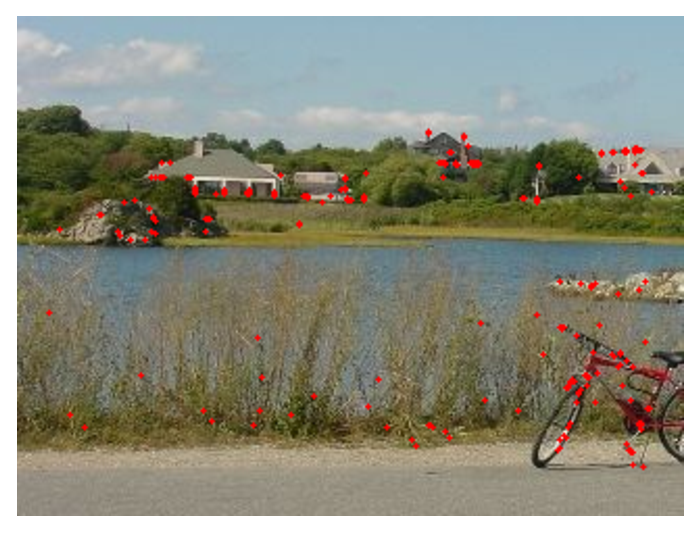
\includegraphics[width=75mm]{./figures/overview/fig2.eps}
        \end{center}
    \end{minipage}
    \begin{minipage}{0.5\hsize}
        \begin{center}
            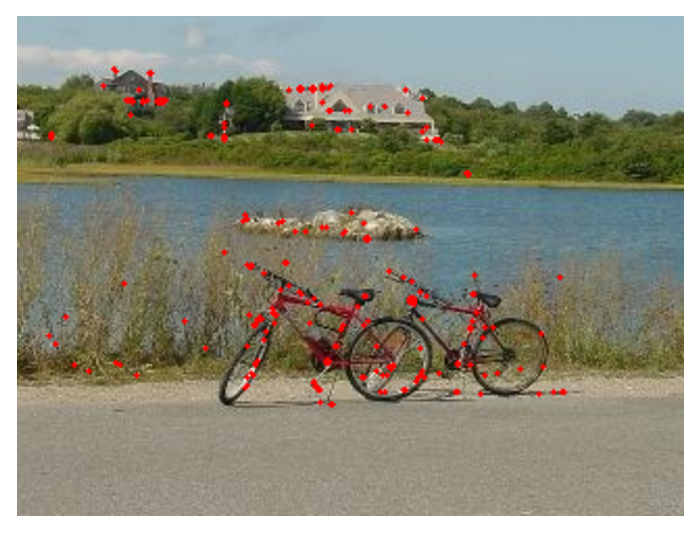
\includegraphics[width=75mm]{./figures/overview/fig3.eps}
        \end{center}
    \end{minipage}
\end{figure}
\begin{figure}[H]
    \begin{center}
        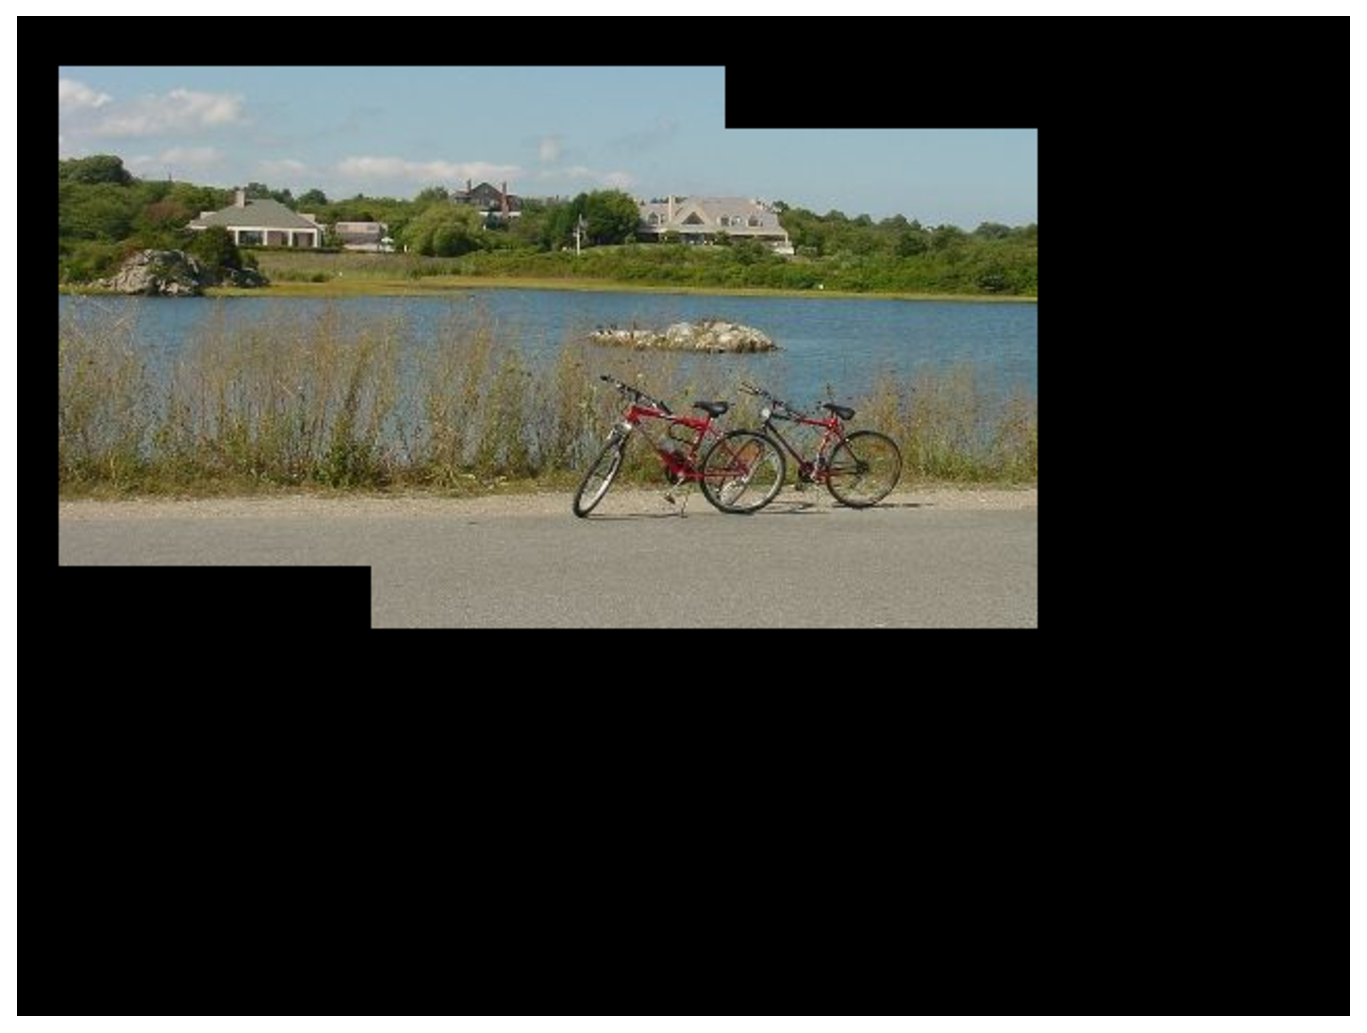
\includegraphics[width=100mm]{./figures/overview/fig4.eps}
    \end{center}
\end{figure}
また,レベル1のデータセット10セットにおけるパノラマ画像作成の成否,および処理時間は以下のようになった.
\begin{table}[H]
    \begin{center}
        \begin{tabular}{ccccc}
            \hline
            Target & Result(default) & Result(FAST) & Time(default) & Time(FAST)\\
            \hline \hline
            1-001 & $\circ$ & $\circ$ & 35.56 & 12.77\\
            1-002 & $\times$ & $\circ$ & 292.36 & 53.93\\
            1-003 & $\times$ & $\circ$ & 3.61 & 3.52\\
            1-004 & $\circ$ & $\circ$ & 215.18 & 47.27\\
            1-005 & $\times$ & $\circ$ & 58.56 & 26.96\\
            1-006 & $\times$ & $\circ$ & 20.92 & 16.25\\
            1-007 & $\times$ & $\circ$ & 295.62 & 55.06\\
            1-008 & $\times$ & $\times$ & 3.78 & 3.47\\
            1-009 & $\circ$ & $\circ$ & 183.84 & 46.63\\
            1-010 & $\times$ & $\times$ & 60.60 & 24.80\\
            \hline
        \end{tabular}
    \end{center}
\end{table}
処理に使用したPCは"MacBook Pro(Core i5,メモリ8GB)"である.


\subsection{課題}
\begin{itemize}
    \setlength{\itemsep}{5mm}
    \item 正答率の向上に関しての課題\par
    \vspace{1mm}
    \quad
    前節で示したように,Level1では8, 10のデータセットで正しくパノラマを作成できなかった.
    これは,重なるべき場所に置いて特徴点が抽出されていなかったためである.
    これは,$t$および$n$の調節によって改善できると考えられる.
    \item 回転,およびスケールへの対応の課題\par
    \vspace{1mm}
    \quad
    本課題で作ったプログラムは,回転およびスケールには正しく対応できない.
    これは特徴点抽出のフェーズに置いて,隣接する2点を抽出してしまうために,マッチングの際にもっとも信頼のおける特徴点2対が隣接するピクセルになり,回転,拡大が正しく計算できない可能性があるためである.(そもそも変換行列を計算する関数は現状本プログラムには組み込まれていない.)
    これを解決するためには,特徴点抽出のフェーズで隣接する特徴点が存在した場合,特徴量の小さい方の特徴点を「間引く」非最大値抑制と言われる処理を行う必要がある.
\end{itemize}

\section{感想}
\begin{itemize}
    \setlength{\itemsep}{5mm}
    \item 濱崎 直紀(馬場口研究室)\\
    担当:プログラミング(サンプルプログラム),レポート作成\par
    \vspace{2mm}
    \quad
    研究の一環などで画像から特徴などを抽出することはあったが,基本的にOpenCVなどの画像処理系ライブラリを用いていたため,実際にその内部で行われていることをしっかり理解していなかった.
    しかし,今回の課題があったことで,数多くある手法の一つではあるが,FASTの内部で行われていることの理解を深めることができた.
    ライブラリの存在により実際に行われていることが曖昧になりがちだったが,そのアルゴリズムを知ることの重要さを感じた.\par\quad
    また,FASTのプログラムを実際に書くことに関してはほぼ貢献できなかったという反省点があるので,次回の課題の際にはグループの一員としての役割をしっかりと果たせるように努めたい.
    \item 永井 智之(井上研究室)\\
    担当:プログラミング(ガウスノイズの実装)\par
    \vspace{2mm}
    \quad
    ガウスノイズの実装を行なったが,FASTの方での実装は行なっておらず,何か結果を示すことは出来なかった.
    問題点として,目標をしっかりと定めずに課題を行なっていたことが挙げられる.\par\quad
    また,FASTの方は中尾くんに任せっきりだったので,次回の課題では班に貢献できるようにしたい.
    \item 中尾 文亮(八木研究室)\\
    担当:プログラミング(FASTの実装)\par
    \vspace{2mm}
    \quad
    今回FASTプログラムを実装したが,高速化のプログラムを省略してしまったり,周囲のピクセルとの輝度比較のプログラムで冗長な書き方をしてしまうなど,主に「処理速度」の点で妥協ののこる実装になってしまった.
    次回の課題では,ただ動けばいいということではなく,速さも求めたプログラムを書きたい.
\end{itemize}


%======================================================================
%		付録
%======================================================================

\clearpage
\appendix
\pagestyle{empty}
% ソースコードの表示に関する設定
\lstset{
    basicstyle={\ttfamily},
    identifierstyle={\small},
    commentstyle={\smallitshape},
    keywordstyle={\small\bfseries},
    ndkeywordstyle={\small},
    stringstyle={\small\ttfamily},
    frame={tb},
    breaklines=true,
    columns=[l]{fullflexible},
    numbers=left,
    xrightmargin=0zw,
    xleftmargin=3zw,
    numberstyle={\scriptsize},
    stepnumber=1,
    numbersep=1zw,
    lineskip=-0.5ex
}
\section{プログラム1}
\begin{lstlisting}[caption=FAST]
    import cv2
    import numpy as np
    
    class FAST:
    
      def __init__(self, t, n):
        self.t = t
        self.n = n 
    
      # カラー画像を引数として、FASTで抽出した特徴点座標をタプルの配列で返す
      def get_img_feature(self, img):
    
        img_feature= []
    
        img = cv2.cvtColor(img, cv2.COLOR_BGR2GRAY)
        height, width = img.shape
    
        for x in range(width):
          for y in range(height):
    
            #上下左右15ピクセルは処理しない(接合時のことを考慮)
            if (
                 x in range(0,15) 
              or x in range(width-15,width) 
              or y in range(0,15) 
              or y in range(height-15,height)
              ):
                continue
    
            standard_brightness = img[y][x] #基準となる明るさ
    
            surrounding_pixels = np.array(
              [
                int(img[y-3][x]),
                int(img[y-3][x+1]),
                int(img[y-2][x+2]),
                int(img[y-1][x+3]),
                int(img[y][x+3]),
                int(img[y+1][x+3]),
                int(img[y+2][x+2]),
                int(img[y+3][x+1]),
                int(img[y+3][x]),
                int(img[y+3][x-1]),
                int(img[y+2][x-2]),
                int(img[y+1][x-3]),
                int(img[y][x-3]),
                int(img[y-1][x-3]),
                int(img[y-2][x-2]),
                int(img[y-3][x-1])
              ]
            )
    
            # #現状これがないほうが早く動くんだよなぁ..
            # #高速化プログラム(本来n>12の時適用)#######################################################
            # brightness_status_array = [0,0]
    
            # for i in [0,4,8,12]:
            #   brightness_status = self.__get_brightness_status(brightness_around_array[i], brightness, self.t)
            #   if brightness_status == "bright":
            #     brightness_status_array[0] += 1 
            #   elif brightness_status == "dark":
            #     brightness_status_array[1] += 1
    
            #   #明るい点が2点の場合break
            #   if not (brightness_status_array[0]>2 or brightness_status_array[1]>2):
            #     continue
            # ######################################################################################
    
            consecutive_num_array = [] #明るさ判断が連続して一致した数の格納用
            consecutive_num_el = 0 #明るさ判断が連続して一致した数の一時保存用
            brightness_status = 0
            brightness_status_before = 0
    
            #0部分のbrightness statusをここで定義
            brightness_status_before = self.__get_brightness_status(surrounding_pixels[0], standard_brightness)
    
            for i in range(16):
    
              #0部分のbrightness statusをここで定義
              brightness_status = self.__get_brightness_status(surrounding_pixels[i], standard_brightness)
    
              #前の要素の明るさが中間値でなく、かつ前の要素と一致する場合
              if brightness_status != 0 and brightness_status_before == brightness_status:
    
                consecutive_num_el += 1
    
              else: #前の要素と明るさに関する要件が一致しない
    
                consecutive_num_array.append(consecutive_num_el)
                consecutive_num_el = 1
              
              #brightness_statusの更新
              brightness_status_before = brightness_status
            
            #最終結果および、最初と最後の足し合わせを末尾に追加
            consecutive_num_array.append(consecutive_num_el)
            consecutive_num_array.append( consecutive_num_array[0] + consecutive_num_array[-1] )
    
            if np.amax(consecutive_num_array) > self.n:
              img_feature.append((x,y))
    
        print("feature detect process finished")
        return img_feature
    
    
      #2画像とその特徴点からもっともマッチした組み合わせを返す
      #(この関数は回転対応のためにちょっと書き換える必要あり)
      def get_best_match_feature(self, img1, img1_features, img2, img2_features):
    
        img1_best_feature = (0,0)
        img2_best_feature = (0,0)
        min_diff = 1000000000
    
        for feature1 in img1_features:
    
          x1,y1 = feature1
    
          for feature2 in img2_features:
    
            x2,y2 = feature2
    
            img1_fraction = img1[y1-10:y1+10, x1-10:x1+10].astype(np.int8).flatten()
            img2_fraction = img2[y2-10:y2+10, x2-10:x2+10].astype(np.int8).flatten()
    
            diff = np.sum(np.abs(img1_fraction-img2_fraction))
    
            if min_diff > diff:
                min_diff = diff
                img1_best_feature = (x1,y1)
                img2_best_feature = (x2,y2)
    
        return (img1_best_feature, img2_best_feature)
    
      #brightness_status取得部分
      def __get_brightness_status (self, target, brightness):
        if target > brightness+self.t:
          return 1
        elif target < brightness-self.t:
          return -1
        else:
          return 0
          
\end{lstlisting}

\clearpage
\section{タイトル}
\begin{lstlisting}[caption=プログラムタイトル]
    if __name__ == '__main__':
        print('これはテスト用プログラムです.')
\end{lstlisting}
\clearpage
\section{プログラム3}
\begin{lstlisting}[caption=サブプログラム]
import cv2
import numpy as np
import fast

class ProcessImg:

  @classmethod
  def join_img(self, img1, img2, img1_feature, img2_feature):

    height1, width1, color1 = img1.shape
    height2, width2, color2 = img2.shape

    x1, y1 = img1_feature
    x2, y2 = img2_feature

    base_img = np.zeros((height1+height2, width1+width2, 3)).astype(np.uint8)
    height,width,color = base_img.shape
    half_width = int(width/2)
    half_height = int(height/2)
    base_img[half_height-y1:half_height+(height1-y1),half_width-x1:half_width+(width1-x1)] = img1
    base_img[half_height-y2:half_height+(height1-y2),half_width-x2:half_width+(width1-x2)] = img2

    return base_img

  @classmethod
  def rotate_img(self, img, angle):
    rotate_matrix = np.array([[np.cos(angle), -np.sin(angle), 0],
                    [np.sin(angle),  np.cos(angle), 0],
                    [        0,          0, 1]])

    H, W, color = img.shape
    WID = int(np.max(img.shape) * 2**0.5)
    e_img = np.zeros((WID, WID, 3)).astype(np.uint8)
    e_img[int((WID-H)/2):int((WID+H)/2),
          int((WID-W)/2):int((WID+W)/2)] = img
    x = np.tile(np.linspace(-1, 1, WID).reshape(1, -1), (WID, 1))
    y = np.tile(np.linspace(-1, 1, WID).reshape(-1, 1), (1, WID))
    p = np.array([[x, y, np.ones(x.shape)]])
    dx, dy, _ = np.sum(p * rotate_matrix.reshape(3, 3, 1, 1), axis=1)
    u = np.clip((dx + 1) * WID / 2, 0, WID-1).astype('i')
    v = np.clip((dy + 1) * WID / 2, 0, WID-1).astype('i')
    return e_img[v, u]


  @classmethod
  def plot_img_feature(self, img, features):

    for feature in features:
      cv2.circle(img, feature, 1, (0, 0, 255), thickness=-1)
    
    return img

\end{lstlisting}

\clearpage
\section{プログラム4}
\begin{lstlisting}[caption=サンプルプログラム(Python)]
import cv2
import math
import numpy as np
import os
import time
os.chdir(os.path.dirname(os.path.abspath(__file__)))


def mosaicGetMin(image3, image4, xmin, xmax, ymin, ymax, tmin, tmax, tstep, width1, height1, width2, height2):
    min = 1.7976931348623157e+308

    t = tmin
    while t < tmax:
        s1 = math.sin(t * math.pi / 180.0)
        c1 = math.cos(t * math.pi / 180.0)
        y = ymin
        while y <= ymax:
            x = xmin
            while x <= xmax:
                print('x:{} y:{} t:{}'.format(x, y, t))
                s = 0
                count = 0
                i = 0
                while i < height2:
                    j = 0
                    while j < width2:
                        # 画像を回転したときのピクセルの位置
                        u = int(math.floor((s1 * i + c1 * j) + x + 0.5))
                        v = int(math.floor((c1 * i - s1 * j) + y + 0.5))
                        # 画像が重ならない部分は誤差を計算しない
                        if u < 0 or u >= width1 or v < 0 or v >= height1:
                            j += 1
                            continue
                        pixelValue1 = image3[v, u]
                        pixelValue2 = image4[i, j]
                        # 二乗誤差の計算
                        tmp = int(pixelValue1[0]) - int(pixelValue2[0])
                        s += tmp * tmp
                        tmp = int(pixelValue1[1]) - int(pixelValue2[1])
                        s += tmp * tmp
                        tmp = int(pixelValue1[2]) - int(pixelValue2[2])
                        s += tmp * tmp
                        count += 1

                        j += 1
                    i += 1

                # 平均二乗誤差の計算
                ave = s / count
                # 平均二乗誤差が最小値より小さい場合はパラメータの更新
                if min > ave:
                    min = ave
                    i_min = y
                    j_min = x
                    t_min = t

                x += 1
            y += 1
        t += tstep
    
    return i_min, j_min, t_min


def mosaicResizeImage(image, re_w, re_h):
    h, w, c = image.shape

    re_image = np.arange(re_w * re_h * 3).reshape(re_h, re_w, 3)

    # 元の画像と新しい画像の大きさの比を計算
    stepx = int(w / re_w)
    stepy = int(h / re_h)

    i = 0
    while i < re_h:
        j = 0
        while j < re_w:
            b = g = r = 0
            count = 0
            k = stepy * i
            while k <= stepy * (i + 1) - 1:
                l = stepx * j
                while l <= stepx * (j + 1) - 1:
                    if k >= h or l >= w:
                        l += 1
                        continue
                    pixelValue = image[k, l]
                    b += pixelValue[0]
                    g += pixelValue[1]
                    r += pixelValue[2]
                    count += 1
                    l += 1
                k += 1
            re_image[i, j][0] = b / count
            re_image[i, j][1] = g / count
            re_image[i, j][2] = r / count
            j += 1
        i += 1

    return re_image


def mosaic(image1, image2):
    # 入力画像の幅と高さを抽出
    h1, w1, c1 = image1.shape
    h2, w2, c2 = image2.shape

    # 1/5に縮小した画像を作成
    image3 = mosaicResizeImage(image1, int(w1/5), int(h1/5))
    image4 = mosaicResizeImage(image2, int(w2/5), int(h2/5))

    # 縮小画像の幅と高さを抽出
    h3, w3, c3 = image3.shape
    h4, w4, c4 = image4.shape

    # 縮小した画像で、画像が最も重なるときのパラメータを概算
    tempy, tempx, tempt = mosaicGetMin(image3, image4, 2, w3-3, 2, h3-3, -15, 15, 2.0, w3, h3, w4, h4)
    # 元の画像でパラメータを計算
    tempy, tempx, tempt = mosaicGetMin(image1, image2, (tempx-1)*5, (tempx+1)*5-1, (tempy-1)*5, (tempy+1)*5-1, tempt-1.0, tempt+1.0, 1.0, w1, h1, w2, h2)

    return tempx, tempy, tempt


if __name__ == '__main__':
    filename1 = 'Level1/1-001-1.jpg'
    filename2 = 'Level1/1-001-2.jpg'

    image1 = cv2.imread(filename1)
    image2 = cv2.imread(filename2)

    start = time.time()

    dx, dy, dt = mosaic(image1, image2)

    elapsed_time = time.time() - start

    print('dx={}'.format(dx))
    print('dy={}'.format(dy))
    print('dt={}'.format(dt))

    print('処理時間:{}'.format(elapsed_time))
    
\end{lstlisting}


\end{document}
